% lvo-so-different-key.tex

\documentclass[tikz]{standalone}
% gentlerain-preamble.tex

\usetikzlibrary{calc, positioning, arrows.meta}

\def\b{bot} % literal string

\newcommand{\client}{\textsl{Client}}
\newcommand{\server}{\textsl{Server}}

\newcommand{\request}{\texttt{req}}
\newcommand{\reply}{\texttt{rep\;}}
\newcommand{\repl}{\texttt{repl\;}}

\newcommand{\so}{\texttt{so}}
\newcommand{\lvo}{\texttt{lvo}}
\newcommand{\rvo}{\texttt{rvo}}

\newcommand{\vs}{\texttt{vs}}
\newcommand{\lvs}{\texttt{lvs}}
\newcommand{\rvs}{\texttt{rvs}}


% send
\newcommand{\send}[9]{
% #1: sender; #2: sender pos; #3: sender event label; #4: sender name
% #5: receiver; #6: receiver pos; #7: receiver event label; #8: receiver name
% #9: label position
  \draw[->]  
  	($(#1)!#2!(#1\b)$) 
		node[#9] (#4) {$#3$}
     to ($(#5)!#6!(#5\b)$) 
     		node[#9] (#8) {$#7$};
}

\begin{document}
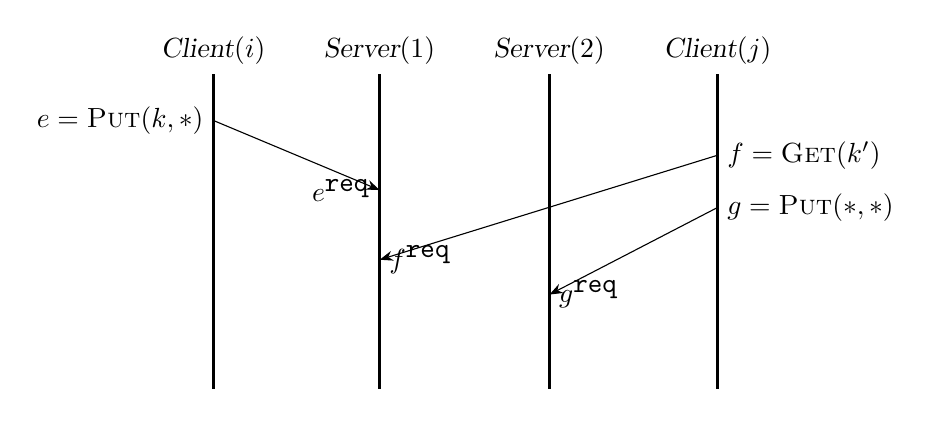
\begin{tikzpicture}[
    >=Stealth, 
    timeline/.style = {very thick}, 
    replica/.style = {align = center},
    node distance = 0.50cm]
  \node[replica] (ci) {$\client(i)$};
  \node[replica, right = of ci] (s) {$\server(1)$};
  \node[replica, right = of s] (s') {$\server(2)$};
  \node[replica, right = of s'] (cj) {$\client(j)$};

  \foreach \r/\rbot in {ci/cibot, s/sbot, s'/s'bot, cj/cjbot} {
    \node[below = 4.0cm of \r] (\rbot) {};
    \draw[timeline] (\r) to (\rbot);
  }

  \send{ci}{0.20}{e = \textsc{Put}(k, \ast)}{e}{s}{0.40}{e^{\texttt{req}}}{ereq}{left}
  \send{cj}{0.30}{f = \textsc{Get}(k')}{}{s}{0.60}{f^{\texttt{req}}}{freq}{right}

  \send{cj}{0.45}{g = \textsc{Put}(\ast, \ast)}{g}{s'}{0.70}{g^{\texttt{req}}}{ereq}{right}
\end{tikzpicture}
\end{document}
